\documentclass[conference]{IEEEtran}
\IEEEoverridecommandlockouts
\usepackage[utf8]{inputenc}
\usepackage[T1]{fontenc}
\usepackage{cite}
\usepackage{amsmath,amssymb}
\usepackage{graphicx}
\usepackage{booktabs}
\usepackage{url}
\usepackage[hidelinks]{hyperref}

\begin{document}

\title{TRM Predict: A Cloud-Native Predictive Analytics System for Exchange-Rate Risk Decisions in Colombia}

\author{
\IEEEauthorblockN{Sebastián Cubides, Nicolás Vergara, Edgar Ruiz}
\IEEEauthorblockA{\textit{Data Engineering and Artificial Intelligence, 5th semester}\\
\textit{University Name}, City, Colombia\\
Integrative Project: Data Mining, Machine Learning and Cloud Computing --- 2026-2}
}

\maketitle

\begin{abstract}
Colombian households that receive remittances and micro, small and medium enterprises (MSMEs) that import goods are exposed to the volatility of the peso--dollar exchange rate (TRM), yet they lack the analytical tools available to large corporations. This proposal presents \emph{TRM Predict}, a cloud-native decision-support system that forecasts, for the next business day, the direction of the TRM, its expected value and the probability of a large move. The data pipeline follows CRISP-DM and integrates the official TRM (open-data API), global market variables, crypto-assets and a web-scraping module that turns financial news headlines into a daily FX-sentiment index. Unsupervised mining (PCA, K-Means, hierarchical clustering, DBSCAN, Apriori and FP-Growth) characterizes market regimes and co-movement rules. Supervised models range from regularized linear models, KNN and SVM to ensembles (Random Forest, AdaBoost, Gradient Boosting) tuned with Grid and Random Search under time-series cross-validation, and explained with SHAP and LIME. The system is deployed on AWS with Terraform: a serverless ingestion layer (EventBridge, Lambda), an S3 data lake replicated to a second region, PostgreSQL on RDS, and a containerized REST API behind an Application Load Balancer with auto-scaling across two availability zones. The project contributes to SDG~8 (target 8.10) and SDG~10 (target 10.c).
\end{abstract}

\begin{IEEEkeywords}
cloud computing, data mining, machine learning, CRISP-DM, ensemble learning, exchange-rate forecasting, sustainable development
\end{IEEEkeywords}

\section{Introduction}
The \emph{Tasa Representativa del Mercado} (TRM) is the official COP/USD exchange rate certified daily by Colombia's Financial Superintendence. It sets the price of imported goods, the value of remittances received by households, and the cost of dollar-denominated debt. Between September 2017 and October 2026 the TRM moved between 2{,}705 (April 2018) and 5{,}061 COP/USD (November 2022), and during 2025 alone it ranged from 3{,}707 to 4{,}417, a swing of 19\%. In our data set, 18\% of trading days show a variation larger than 1\%.

Large firms manage this risk with treasury desks and derivatives; households and MSMEs usually decide on intuition. Remittances to Colombia exceeded USD~11.8 billion in 2024 according to the central bank~\cite{banrep_remesas}, so even small improvements in \emph{when} a family converts its dollars translate into meaningful income. The project therefore aligns with the United Nations 2030 Agenda~\cite{un2015}: SDG~8 (target 8.10, access to financial services) and SDG~10 (target 10.c, reducing the cost of remittances).

\section{Problem Statement}
\textbf{Problem.} Non-expert economic agents in Colombia have no accessible, transparent and continuously updated tool to estimate the short-term behavior and risk of the TRM. \textbf{Users.} (i) Households receiving remittances; (ii) importing MSMEs that must buy dollars; (iii) instructors and students of financial literacy programs. \textbf{Question.} Using public data available before the publication of the next TRM, can we (a) estimate the probability that it rises, (b) estimate its expected value, and (c) anticipate days of abnormally large moves, with performance verifiably better than naive baselines, and explain each prediction?

Exchange rates are notoriously hard to forecast: Meese and Rogoff showed that structural models do not beat a random walk out of sample~\cite{meese1983}. The project therefore treats the random walk and the majority class as mandatory baselines, and values rigor and honest evaluation over model complexity.

\section{Related Work}
Machine learning applied to financial markets has been surveyed extensively. Henrique \emph{et al.}~\cite{henrique2019} review more than 50 studies and report that support vector machines and neural networks dominate, with ensemble methods gaining ground. Sezer \emph{et al.}~\cite{sezer2020} cover deep learning for financial time series and highlight the lack of interpretability and reproducibility. Most studies target major currency pairs or stock indices, rarely emerging-market currencies such as the COP, and few provide a deployable, explainable service for non-expert users. This project addresses that gap by combining (i) Colombia-specific drivers (oil price, regional peer currencies, local news sentiment), (ii) interpretable ensembles with SHAP~\cite{lundberg2017} and LIME~\cite{ribeiro2016}, and (iii) a reproducible cloud deployment built with Infrastructure as Code.

\section{Proposed System}
Fig.~\ref{fig:arch} shows the end-to-end system. Every business day at 18:30 (Colombia time), after the TRM is published, an EventBridge rule triggers an \emph{ingestion} Lambda function. It calls the open-data API of the TRM, Yahoo Finance (Brent, DXY, US 10-year yield, VIX, S\&P~500, USD/MXN, USD/BRL and USD/COP spot) and the Binance API (BTC, ETH), and scrapes the headlines of \emph{La Rep\'ublica}. The resulting JSON bundle lands in the raw zone of an S3 data lake, and that event triggers an \emph{ETL} Lambda that upserts the records into PostgreSQL. The models are trained offline with the CRISP-DM pipeline and published to S3. A FastAPI service in Docker loads the model and serves predictions, what-if scenarios and a web dashboard.

\begin{figure*}[t]
\centering
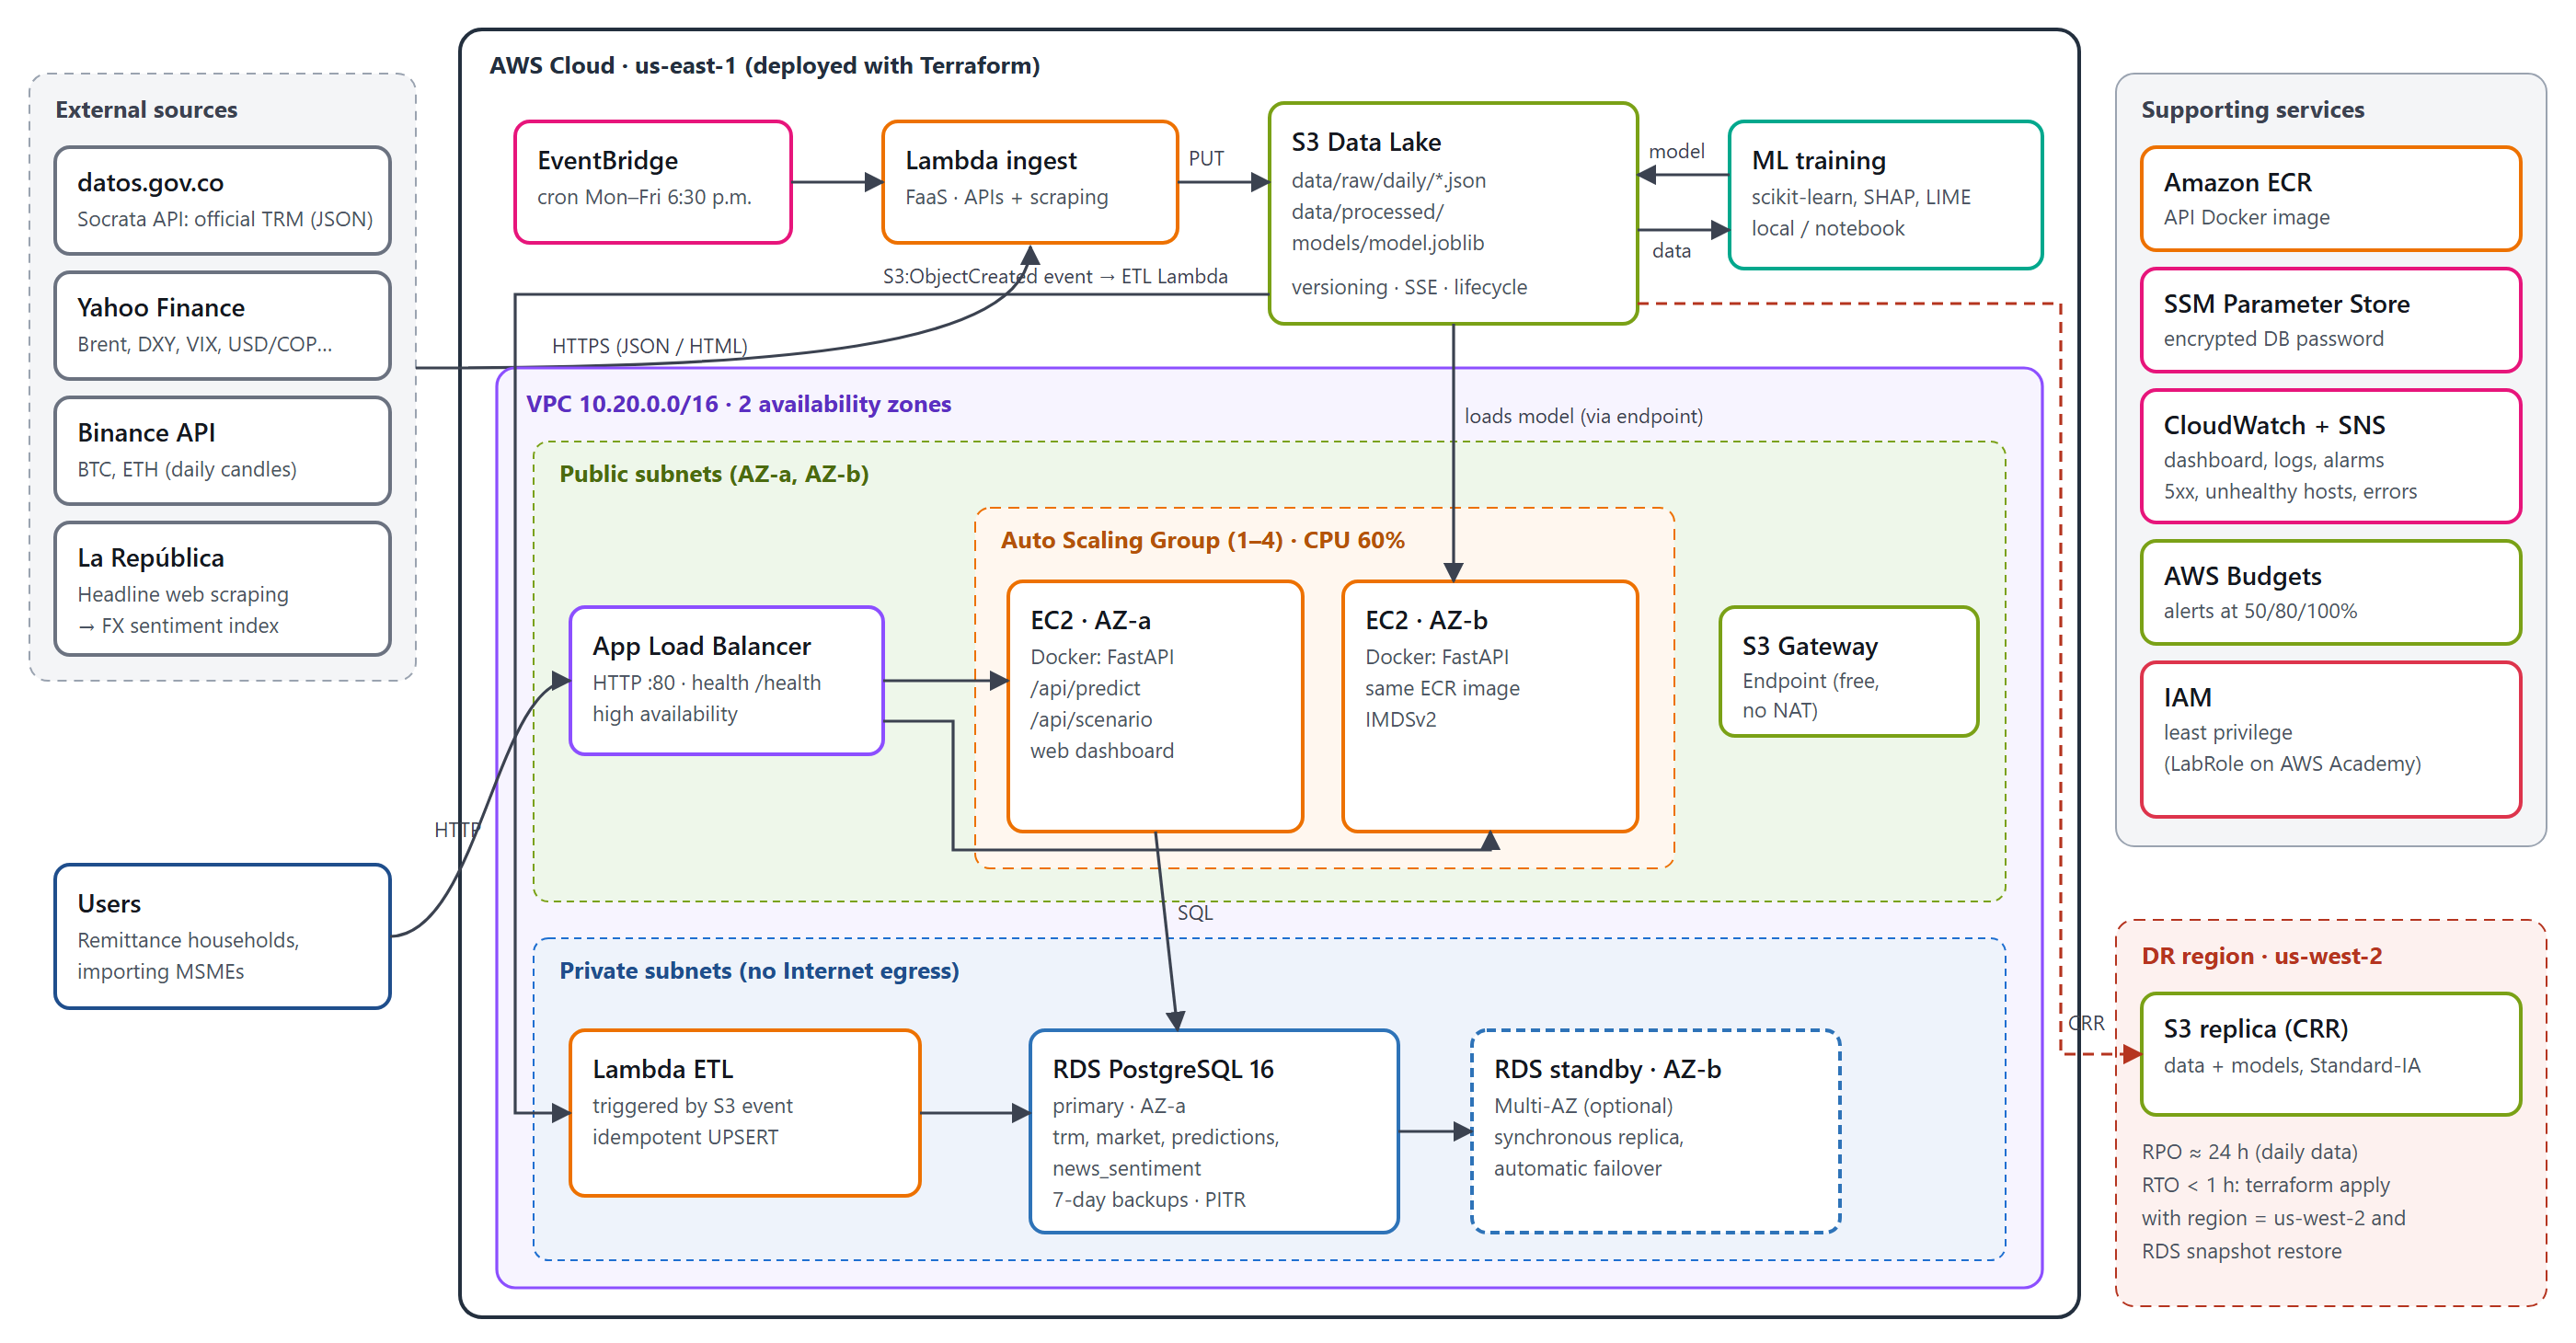
\includegraphics[width=\textwidth]{../arquitectura_en.png}
\caption{TRM Predict architecture on AWS: serverless ingestion, S3 data lake with cross-region replication, RDS in private subnets, and an auto-scaled API behind an Application Load Balancer in two availability zones.}
\label{fig:arch}
\end{figure*}

\section{Cloud Architecture}
\textbf{Provider and deployment model.} Public cloud on AWS (us-east-1), chosen for its course alignment, AWS Academy credits and mature Terraform provider; a second region (us-west-2) is used for disaster recovery. \textbf{Service models.} IaaS (EC2 instances for the API), PaaS (RDS PostgreSQL, Application Load Balancer, ECR), FaaS (Lambda for ingestion and ETL) and SaaS (the dashboard consumed by end users), following the NIST definitions~\cite{nist800145}.

\textbf{Scalability.} An Auto Scaling Group (1--4 \texttt{t3.micro} instances) with a target-tracking policy at 60\% average CPU; RDS storage auto-scales from 20 to 50~GB. \textbf{High availability.} The ALB spans two availability zones and routes only to instances that pass the \texttt{/health} check; the ASG replaces unhealthy instances automatically; RDS can run Multi-AZ with synchronous standby and automatic failover. \textbf{Disaster recovery.} S3 versioning plus Cross-Region Replication of data and models; RDS automated backups (7 days, point-in-time recovery); the whole stack can be rebuilt in the DR region with \texttt{terraform apply}. Targets: RPO $\approx$ 24~h, RTO $<$ 1~h (backup-and-restore strategy~\cite{aws_wellarchitected}). \textbf{Security.} RDS and the ETL Lambda live in private subnets without Internet access; S3 is reached through a free VPC gateway endpoint (avoiding a NAT gateway); the database password is stored encrypted in SSM Parameter Store; instances enforce IMDSv2 and accept traffic only from the ALB. \textbf{IaC.} All resources (VPC, subnets, security groups, S3, RDS, ALB, ASG, Lambda, EventBridge, CloudWatch alarms and dashboard, AWS Budgets) are declared in Terraform~\cite{terraform_aws}, versioned in the repository and validated with \texttt{terraform validate}.

\section{Data Mining Pipeline}
The pipeline follows the KDD process~\cite{fayyad1996} organized with CRISP-DM~\cite{wirth2000}. \textbf{Acquisition.} Four heterogeneous sources and formats: Socrata JSON API (8{,}370 TRM records since 1991), Yahoo Finance JSON stored as CSV (8 series), Binance JSON (2 crypto-assets) and HTML scraping. The scraper has a concrete purpose: it counts dollar-related headlines and computes a lexicon-based FX-sentiment score, qualitative information that no API provides.

\textbf{Preparation.} Type casting, duplicate and invalid-date removal, positivity checks, IQR-based outlier audit of returns, and a strict \texttt{merge\_asof} that only uses market data published \emph{before} each TRM date to prevent look-ahead leakage. The final data set has 2{,}159 daily observations (Sep.~2017--Oct.~2026) and 43 features: log-returns and lags of the TRM, 5- and 20-day volatility, moving-average ratio, z-score, calendar variables, 1- and 5-day returns and 20-day volatility of each market, and the gap between the last spot quote and the current TRM.

\textbf{EDA.} Descriptive statistics, distribution tests, correlation heat maps and rolling correlations. TRM returns are leptokurtic (excess kurtosis 3.0, Jarque--Bera $p<10^{-100}$) and show positive first-order autocorrelation (0.17), consistent with the TRM being a daily volume-weighted average.

\textbf{Feature engineering and unsupervised mining.} PCA needs 26 of 43 components to retain 90\% of the variance: the features are only weakly redundant, and the first two components represent momentum of the peso and of peer currencies (PC1) and global volatility (PC2). K-Means (with $k$ chosen by the elbow and silhouette methods, $k=3$) and Ward hierarchical clustering segment market \emph{regimes} (risk-off, risk-on and high volatility). The regimes overlap (silhouette 0.12), so they are used as context rather than as hard classes; DBSCAN~\cite{ester1996} flags 57 anomalous days (45 of them in 2020), on which the next-day TRM volatility is 1.7 times higher. Apriori~\cite{agrawal1994} and FP-Growth~\cite{han2000} over discretized daily moves yield interpretable rules, for example \{Brent up, DXY down\} $\Rightarrow$ TRM down (confidence 0.63, lift 1.22) and \{USD/BRL up, USD/MXN up, VIX up\} $\Rightarrow$ TRM up (confidence 0.60, lift 1.24).

\section{Machine Learning Model}
Three supervised tasks share the same feature matrix: (1) \emph{direction} classification (TRM up/down), (2) \emph{risk} classification (next absolute return above the 75th percentile of the training set), and (3) \emph{regression} of the next log-return, from which the expected TRM is derived. All models are scikit-learn~\cite{pedregosa2011} pipelines (scaling, optional feature selection and polynomial expansion). Candidates: linear, polynomial+Ridge, Ridge, Lasso and Elastic Net regression; logistic regression, KNN and SVM classifiers; and the ensembles Random Forest~\cite{breiman2001}, AdaBoost~\cite{freund1997} and Gradient Boosting~\cite{friedman2001}. Hyperparameters are tuned with \texttt{GridSearchCV} (linear models, KNN, SVM, AdaBoost) and \texttt{RandomizedSearchCV}~\cite{bergstra2012} (Random Forest, Gradient Boosting) using 5-fold \texttt{TimeSeriesSplit}. The final model is selected by cross-validation score, never by the test score, and is then judged on computational cost and interpretability. Global explanations use TreeSHAP and feature importance; local explanations of the latest prediction use LIME.

\section{Methodology and Work Plan}
\textbf{Phases} (aligned with the course units): F1 problem definition and acquisition (weeks 1--3); F2 EDA and feature engineering (4--6); F3 modeling and evaluation (7--10); F4 cloud design and IaC deployment (8--12); F5 integration, cost analysis, IEEE paper and poster (13--16).
\textbf{Validation.} Chronological 80/20 split (test period Dec.~2024--Oct.~2026), time-series cross-validation, and mandatory baselines: random walk (RMSE) and majority class (accuracy). Metrics: ROC-AUC, accuracy and F1 for classification; RMSE, MAE, $R^2$, RMSE ratio to the random walk and directional accuracy for regression; silhouette and Davies--Bouldin for clustering; support, confidence and lift for rules; latency, availability and cost for the cloud layer.
\textbf{Preliminary results.} A first full run (Table~\ref{tab:prelim}) shows that only the ensembles beat chance on the test period: for direction, Random Forest and Gradient Boosting reach a ROC-AUC of 0.55--0.57, versus 0.47--0.50 for logistic regression, KNN and SVM, which points to non-linear interactions among drivers. For the risk task the ensembles reach an AUC of 0.59. The Gradient Boosting regressor lowers the random-walk RMSE by 2.4\%. Direction accuracy (53.2\%) does not yet beat the majority class (54.6\%); closing that gap is the main target of Phase~3, through probability calibration, decision thresholds and the scraped sentiment feature. According to SHAP, the most influential variables are the spot--TRM gap, the last TRM return and the daily change of the DXY.

\begin{table}[t]
\caption{Preliminary test results (Dec.~2024--Oct.~2026, $n=432$)}
\label{tab:prelim}
\centering
\begin{tabular}{@{}lccc@{}}
\toprule
Model & AUC dir. & AUC risk & RMSE/RW \\
\midrule
Logistic / Ridge & 0.497 & 0.549 & 0.997 \\
KNN & 0.474 & 0.571 & -- \\
SVM & 0.490 & 0.562 & -- \\
Random Forest & 0.555 & 0.585 & 0.987 \\
AdaBoost & 0.541 & 0.557 & -- \\
Gradient Boosting & \textbf{0.566} & \textbf{0.586} & \textbf{0.976} \\
\bottomrule
\end{tabular}
\end{table}
\textbf{Risks.} Weak predictability of FX (mitigated with honest baselines and the risk task); changes in website structure (scraper isolated, with failures that do not stop numeric ingestion); AWS Academy restrictions on IAM (Terraform supports the existing \texttt{LabRole}); cost overruns (AWS Budgets alerts and \texttt{terraform destroy} after each session).

\section{Expected Outcomes}
(i) A public repository with the CRISP-DM pipeline, trained models, Terraform scripts and the final data set; (ii) a live system on AWS (REST API and dashboard) with demonstrable auto-scaling, failover and cross-region replication; (iii) a model report with baselines, SHAP and LIME explanations; (iv) the final IEEE paper in English and Spanish, and an A1 poster; (v) a backup demo video.

\section{Expected Resource Usage and Costs}
Table~\ref{tab:cost} summarizes the on-demand monthly estimate in us-east-1. Running 24/7 would cost about USD~64 per month. Because the stack is created and destroyed with Terraform, the expected cost for the whole semester (about 40 development hours, one day of failover tests and one week of continuous operation for the defense) is about USD~21, within AWS Academy credits. Avoiding a NAT gateway through the S3 endpoint saves about USD~33 per month.

\begin{table}[t]
\caption{Estimated monthly cost (USD, on-demand, us-east-1, 24/7)}
\label{tab:cost}
\centering
\begin{tabular}{@{}lr@{}}
\toprule
Service (configuration) & USD/month \\
\midrule
Application Load Balancer (low traffic) & 17.0 \\
EC2: 2 $\times$ t3.micro + 16 GB gp3 & 16.5 \\
Public IPv4 addresses (4) & 14.6 \\
RDS PostgreSQL db.t4g.micro + 20 GB & 14.0 \\
S3 + cross-region replica, ECR & 0.2 \\
Lambda, EventBridge, SSM & 0.0 \\
CloudWatch, data transfer & 1.3 \\
\midrule
\textbf{Total (dev, Single-AZ)} & \textbf{63.6} \\
Production (Multi-AZ, up to 4 instances) & 78--95 \\
\bottomrule
\end{tabular}
\end{table}

\begin{thebibliography}{99}
\bibitem{un2015} United Nations, ``Transforming our world: The 2030 Agenda for Sustainable Development,'' A/RES/70/1, 2015.
\bibitem{banrep_remesas} Banco de la Rep\'ublica de Colombia, ``Ingresos de remesas de trabajadores en Colombia,'' Estad\'isticas del sector externo, 2025. [Online]. Available: \url{https://www.banrep.gov.co}
\bibitem{meese1983} R. A. Meese and K. Rogoff, ``Empirical exchange rate models of the seventies: Do they fit out of sample?'' \emph{J. Int. Econ.}, vol. 14, no. 1--2, pp. 3--24, 1983.
\bibitem{henrique2019} B. M. Henrique, V. A. Sobreiro, and H. Kimura, ``Literature review: Machine learning techniques applied to financial market prediction,'' \emph{Expert Syst. Appl.}, vol. 124, pp. 226--251, 2019.
\bibitem{sezer2020} O. B. Sezer, M. U. Gudelek, and A. M. Ozbayoglu, ``Financial time series forecasting with deep learning: A systematic literature review: 2005--2019,'' \emph{Appl. Soft Comput.}, vol. 90, Art. no. 106181, 2020.
\bibitem{lundberg2017} S. M. Lundberg and S.-I. Lee, ``A unified approach to interpreting model predictions,'' in \emph{Adv. Neural Inf. Process. Syst. (NeurIPS)}, vol. 30, 2017, pp. 4765--4774.
\bibitem{ribeiro2016} M. T. Ribeiro, S. Singh, and C. Guestrin, ```Why should I trust you?': Explaining the predictions of any classifier,'' in \emph{Proc. 22nd ACM SIGKDD Int. Conf. Knowl. Discov. Data Min.}, 2016, pp. 1135--1144.
\bibitem{nist800145} P. Mell and T. Grance, ``The NIST definition of cloud computing,'' NIST, Gaithersburg, MD, USA, Special Publication 800-145, 2011.
\bibitem{aws_wellarchitected} Amazon Web Services, ``Disaster recovery of workloads on AWS: Recovery in the cloud,'' AWS Whitepaper, 2021. [Online]. Available: \url{https://docs.aws.amazon.com/whitepapers/latest/disaster-recovery-workloads-on-aws/}
\bibitem{terraform_aws} HashiCorp, ``Terraform AWS provider documentation,'' 2026. [Online]. Available: \url{https://registry.terraform.io/providers/hashicorp/aws/latest/docs}
\bibitem{fayyad1996} U. Fayyad, G. Piatetsky-Shapiro, and P. Smyth, ``From data mining to knowledge discovery in databases,'' \emph{AI Mag.}, vol. 17, no. 3, pp. 37--54, 1996.
\bibitem{wirth2000} R. Wirth and J. Hipp, ``CRISP-DM: Towards a standard process model for data mining,'' in \emph{Proc. 4th Int. Conf. Pract. Appl. Knowl. Discov. Data Min.}, 2000, pp. 29--39.
\bibitem{ester1996} M. Ester, H.-P. Kriegel, J. Sander, and X. Xu, ``A density-based algorithm for discovering clusters in large spatial databases with noise,'' in \emph{Proc. 2nd Int. Conf. Knowl. Discov. Data Min. (KDD)}, 1996, pp. 226--231.
\bibitem{agrawal1994} R. Agrawal and R. Srikant, ``Fast algorithms for mining association rules,'' in \emph{Proc. 20th Int. Conf. Very Large Data Bases (VLDB)}, 1994, pp. 487--499.
\bibitem{han2000} J. Han, J. Pei, and Y. Yin, ``Mining frequent patterns without candidate generation,'' in \emph{Proc. ACM SIGMOD Int. Conf. Manag. Data}, 2000, pp. 1--12.
\bibitem{pedregosa2011} F. Pedregosa \emph{et al.}, ``Scikit-learn: Machine learning in Python,'' \emph{J. Mach. Learn. Res.}, vol. 12, pp. 2825--2830, 2011.
\bibitem{breiman2001} L. Breiman, ``Random forests,'' \emph{Mach. Learn.}, vol. 45, no. 1, pp. 5--32, 2001.
\bibitem{freund1997} Y. Freund and R. E. Schapire, ``A decision-theoretic generalization of on-line learning and an application to boosting,'' \emph{J. Comput. Syst. Sci.}, vol. 55, no. 1, pp. 119--139, 1997.
\bibitem{friedman2001} J. H. Friedman, ``Greedy function approximation: A gradient boosting machine,'' \emph{Ann. Statist.}, vol. 29, no. 5, pp. 1189--1232, 2001.
\bibitem{bergstra2012} J. Bergstra and Y. Bengio, ``Random search for hyper-parameter optimization,'' \emph{J. Mach. Learn. Res.}, vol. 13, pp. 281--305, 2012.
\end{thebibliography}

\end{document}
